\documentclass[onecolumn]{article}

%\makeatletter\if@twocolumn\PassOptionsToPackage{switch}{lineno}\else\fi\makeatother

%Publisher: UKM_PUBLISHER 
%Template Provided By: Typeset
%\usepackage{amsfonts,amssymb,amsbsy,latexsym,amsmath,tabulary,graphicx,times,xcolor}
%\usepackage[T1]{fontenc}

\usepackage{graphicx}

%% use xelatex
%
%\usepackage{fontspec}
%\usepackage{unicode-math}
%\setmainfont{Times New Roman}
%\setmathfont{Cambria Math}
%\setsansfont{Arial}

\RequirePackage[utf8]{inputenc}
\RequirePackage[T1]{fontenc}
\RequirePackage{newtxtext}
\RequirePackage{newtxmath}
\RequirePackage{helvet}
\RequirePackage{times}


%%%%%%%%%%%%%%%%%%%%%%%%%%%%%%%%%%%%%%%%%%%%%%%%%%%%%%%%%%%%%%%%%%%%%%%%%%
% Following additional macros are required to function some 
% functions which are not available in the class used.
%%%%%%%%%%%%%%%%%%%%%%%%%%%%%%%%%%%%%%%%%%%%%%%%%%%%%%%%%%%%%%%%%%%%%%%%%%
\usepackage{url,multirow,morefloats,floatflt,cancel,tfrupee}
\usepackage{url}
\usepackage{colortbl}
\usepackage{xcolor}
\usepackage{pifont}
\usepackage[nointegrals]{wasysym}
\urlstyle{rm}

\usepackage[top=1in,bottom=1in,left=1in,right=1in,paperwidth=8.50in,paperheight=11.0in]{geometry}
\usepackage{caption,fancyhdr,abstract}
\captionsetup[figure]{name=FIGURE,labelsep=period}
\captionsetup[table]{name=TABLE,labelsep=period}


%\fancypagestyle{headings}{\renewcommand{\headrulewidth}{0pt}\fancyhf{}\fancyfoot[C]{\thepage}\fancyhead[C]{\journalTitle}}\pagestyle{headings}

%\fancypagestyle{plain}{\renewcommand{\headrulewidth}{0pt}\fancyhf{}\fancyfoot[C]{\thepage}\fancyhead[C]{\journalTitle}}

\usepackage{endnotes}
\let\footnote=\endnote


\def\floatpagefraction{0.8} 
\def\dblfloatpagefraction{0.8}
\def\style#1#2{#2}
\def\xxxguillemotleft{\fontencoding{T1}\selectfont\guillemotleft}
\def\xxxguillemotright{\fontencoding{T1}\selectfont\guillemotright}

\newif\ifmultipleabstract\multipleabstractfalse%
\newenvironment{typesetAbstractGroup}{}{}%

%%%%%%%%%%%%%%%%%%%%%%%%%%%%%%%%%%%%%%%%%%%%%%%%%%%%%%%%%%%%%%%%%%%%%%%%%%



\linespread{1.5}                 
\def\floatpagefraction{0.8}

\setlength{\parindent}{1.4pc}
\usepackage[noindentafter,explicit]{titlesec}
\setlength\columnsep{1.5pc}



\usepackage{textcase}
\titleformat{\section}[hang]{\NormalBaseline\fontsize{13}{15}\selectfont\centering}
{\thesection.}
{6pt}
{\noindent\MakeTextUppercase{#1}}
[]
\titleformat{\subsection}[hang]{\NormalBaseline\fontsize{11}{12.5}\selectfont}
{\thesubsection.}
{6pt}
{\MakeTextUppercase{#1}}
[]
\titleformat{\subsubsection}[runin]{\NormalBaseline\itshape}
{\hspace{24pt}\theparagraph)}
{6pt}
{\indent#1}
[:]
\titleformat{\paragraph}[runin]{\NormalBaseline\itshape}
{\hspace{24pt}\theparagraph)}
{6pt}
{\indent#1}
[:]
\titleformat{\subparagraph}[runin]{\NormalBaseline}
{\thesubsubsection}
{6pt}
{\indent#1}
[]

%\titlespacing{\section}{0pt}{1.5\baselineskip}{.2\baselineskip}
\titlespacing{\section}{0pt}{1.5\baselineskip}{.4\baselineskip}  
\titlespacing{\subsection}{0pt}{1.5\baselineskip}{.4\baselineskip}  
\titlespacing{\subsubsection}{0pt}{1.5\baselineskip}{.4\baselineskip}  
\titlespacing{\paragraph}{0pt}{.5\baselineskip}{10pt}  
\titlespacing{\subparagraph}{0pt}{.5\baselineskip}{10pt}


\renewenvironment{abstract}
{\trivlist\item[]\leftskip1pt\par\itshape{\centering\itshape ABSTRACT\\\noindent }\ignorespaces}{\endtrivlist\vspace*{-12pt}}


\def\NormalBaseline{\def\baselinestretch{1.1}}

\makeatletter
\AtBeginDocument{\@ifpackageloaded{textcomp}{}{\usepackage{textcomp}}}
\makeatother


\makeatletter
%%%For Table column width calculation.
\def\mcWidth#1{\csname TY@F#1\endcsname+\tabcolsep}

%%Hacking center and right align for table
\def\cAlignHack{\rightskip\@flushglue\leftskip\@flushglue\parindent\z@\parfillskip\z@skip}
\def\rAlignHack{\rightskip\z@skip\leftskip\@flushglue \parindent\z@\parfillskip\z@skip}

%Etal definition in references
\@ifundefined{etal}{\def\etal{\textit{et~al}}}{}

\if@twocolumn\usepackage{dblfloatfix}\fi
\usepackage{ifxetex}
\ifxetex\else\if@twocolumn\@ifpackageloaded{stfloats}{}{\usepackage{dblfloatfix}}\fi\fi

\AtBeginDocument{
\expandafter\ifx\csname eqalign\endcsname\relax
\def\eqalign#1{\null\vcenter{\def\\{\cr}\openup\jot\m@th
  \ialign{\strut$\displaystyle{##}$\hfil&$\displaystyle{{}##}$\hfil
      \crcr#1\crcr}}\,}
\fi
}

%For fixing hardfail when unicode letters appear inside table with endfloat
\AtBeginDocument{%
  \@ifpackageloaded{endfloat}%
   {\renewcommand\efloat@iwrite[1]{\immediate\expandafter\protected@write\csname efloat@post#1\endcsname{}}}{\newif\ifefloat@tables}%
}%

\def\BreakURLText#1{\@tfor\brk@tempa:=#1\do{\brk@tempa\hskip0pt}}
\let\lt=<
\let\gt=>
\def\processVert{\ifmmode|\else\textbar\fi}
\let\processvert\processVert

\@ifundefined{subparagraph}{
\def\subparagraph{\@startsection{paragraph}{5}{2\parindent}{0ex plus 0.1ex minus 0.1ex}%
{0ex}{\normalfont\small\itshape}}%
}{}

% These are now gobbled, so won't appear in the PDF.
\newcommand\role[1]{\unskip}
\newcommand\aucollab[1]{\unskip}
  
\@ifundefined{tsGraphicsScaleX}{\gdef\tsGraphicsScaleX{1}}{}
\@ifundefined{tsGraphicsScaleY}{\gdef\tsGraphicsScaleY{.9}}{}
% To automatically resize figures to fit inside the text area
\def\checkGraphicsWidth{\ifdim\Gin@nat@width>\linewidth
	\tsGraphicsScaleX\linewidth\else\Gin@nat@width\fi}

\def\checkGraphicsHeight{\ifdim\Gin@nat@height>.9\textheight
	\tsGraphicsScaleY\textheight\else\Gin@nat@height\fi}

\def\fixFloatSize#1{}
%\@ifundefined{processdelayedfloats}{\setbox0=\hbox{\includegraphics{#1}}\ifnum\wd0<\columnwidth\relax\renewenvironment{figure*}{\begin{figure}}{\end{figure}}\fi}{}}
\let\ts@includegraphics\includegraphics

\def\inlinegraphic[#1]#2{{\edef\@tempa{#1}\edef\baseline@shift{\ifx\@tempa\@empty0\else#1\fi}\edef\tempZ{\the\numexpr(\numexpr(\baseline@shift*\f@size/100))}\protect\raisebox{\tempZ pt}{\ts@includegraphics{#2}}}}

\renewcommand{\includegraphics}[1]{\ts@includegraphics[width=\checkGraphicsWidth]{#1}}
\AtBeginDocument{\def\includegraphics{\@ifnextchar[{\ts@includegraphics}{\ts@includegraphics[width=\checkGraphicsWidth,height=\checkGraphicsHeight,keepaspectratio]}}}

\DeclareMathAlphabet{\mathpzc}{OT1}{pzc}{m}{it}

\def\URL#1#2{\@ifundefined{href}{#2}{\href{#1}{#2}}}

%%For url break
\def\UrlOrds{\do\*\do\-\do\~\do\'\do\"\do\-}%
\g@addto@macro{\UrlBreaks}{\UrlOrds}



\edef\fntEncoding{\f@encoding}
\def\EUoneEnc{EU1}
\makeatother



\makeatletter

\def\author#1{\gdef\@author{\hskip-\dimexpr(\tabcolsep)\hskip1pt\parbox{\dimexpr\textwidth-1pt}{\fontsize{11}{13}\selectfont\raggedright\centering #1}}}

\def\title#1{\gdef\@title{\fontsize{14}{16}\selectfont\raggedright\centering{\bfseries#1}~\\{\textit{\fontsize{12}{14}\selectfont\malaytitle}}}}

\let\@articletype\@empty 
\def\articletype#1{\gdef\@articletype{{\fontsize{13}{15}\selectfont #1}}}


 



\makeatother

\date{}


%% all float at the end of document
%\usepackage[tablesfirst]{endfloat}

\usepackage[authoryear,sort&compress]{natbib}
%\renewcommand{\bibfont}{\SingleSpacing}
\setlength{\bibsep}{\baselineskip}
\setlength{\bibhang}{12.5mm}
\setcitestyle{aysep={}}

\setcounter{secnumdepth}{0}

%% ??
\usepackage{float}



\begin{document}


\def\authorCount{1}
\def\affCount{1}

\def\journalTitle{GEMA Online{\textsuperscript{\textregistered}} Journal of Language Studies}

\title{UKM Cyber-range: Issues and Challenges}
\def\malaytitle{}
\def\articletype{}
\author{Mohd Zamri Murah}
\maketitle
%\clearpage 
% \begin{center}\textbf{\fontsize{14pt}{16pt}\selectfont 
% \title{Success A Habit}\def\malaytitle{()}
% \def\articletype{}}\end{center}

\begin{abstract}
Cyber-range is a virtual environemnt consist of networks, nodes and 
etc. C

\end{abstract}

%%\def\keywordstitle{Keywords}
\vspace{1mm}
\smallskip\noindent\textbf{Keywords: }\textit{student; performance}
    
\section*{Introduction}

Cyber range is a virtual environment for teaching and learning cyber security. Many organization has used cyber range for teaching and learning. However, the cost of building a cyber range is expensive.

Important to have cyber range.

Benefit of cyber range.


\section{Literature review}

\section{Method}

\section{Results}

\section{Conclusion}




\bgroup
%\fixFloatSize{images/298377c4-2e5e-42fe-a79f-1ffa57ed81ce-uread-braille.jpg}
\begin{figure*}[!htbp]
\centering 
\includegraphics{images/298377c4-2e5e-42fe-a79f-1ffa57ed81ce-uread-braille.jpg}
\caption{{Reading Braille}}
\label{f-056fed0128b2}
\end{figure*}
\egroup



%\fixFloatSize{images/298377c4-2e5e-42fe-a79f-1ffa57ed81ce-uread-braille.jpg}
\begin{figure}[!ht]
\centering 

\includegraphics{images/298377c4-2e5e-42fe-a79f-1ffa57ed81ce-uread-braille.jpg}
\caption{{Reading Braille}}
\label{f-056fed0128b2}
\end{figure}


\section*{Methods}
Nullam iaculis sed dui eu placerat\unskip~\cite{572698:13280034} . Etiam
sit amet maximus tortor, quis suscipit turpis. Sed scelerisque arcu sapien.
Donec eu neque at libero interdum egestas nec non dui. Phasellus eu
imperdiet turpis, sit amet imperdiet tellus. Fusce eget eleifend enim.
Praesent eros lorem, tempus sed purus id, lobortis euismod quam.
Suspendisse nec finibus elit. Sed vitae ex vel ipsum semper elementum.
Maecenas placerat elit in dapibus cursus.

Interdum et malesuada fames ac ante ipsum primis in faucibus. Curabitur
viverra at lorem dignissim lacinia. Aliquam finibus a ante ut semper. Fusce
leo eros, venenatis vitae ornare et, luctus vel elit. Sed dictum rutrum
tellus quis venenatis\unskip~\cite{572698:13280063} . Mauris in erat non
lorem ullamcorper aliquet. In pharetra sapien orci, nec dignissim augue
congue vitae. Duis vehicula nibh erat, eget consequat lorem consequat ut.


    
\section*{Results}
Pellentesque luctus erat non magna porta, sit amet malesuada augue
vestibulum. Pellentesque ut felis ultricies, volutpat massa non, dictum
sapien. Sed eu lectus at tellus egestas tincidunt sit amet ut erat. Quisque
convallis, ipsum sit amet vestibulum fermentum, magna lectus finibus ipsum,
consectetur feugiat urna neque ac tellus. In hendrerit interdum leo ac
dictum. Nulla eu lacus elit. Donec congue ex quis velit feugiat rhoncus. Ut
a felis nec neque luctus pharetra egestas faucibus nibh. Nullam gravida
scelerisque massa, ac fermentum ex eleifend ut.

Nam dapibus fringilla quam a iaculis. Donec quis arcu quis velit congue
auctor. Class aptent taciti sociosqu ad litora torquent per conubia nostra,
per inceptos himenaeos. Phasellus dignissim lacus non lorem posuere, vitae
vestibulum ante venenatis. Duis interdum vitae dolor vitae rutrum. Aenean
non eros vel risus mattis imperdiet. Sed dolor sapien, gravida sit amet
porta in, gravida in urna. Vestibulum vehicula vulputate orci nec aliquet.
Donec a felis a lacus lacinia suscipit a accumsan neque. Nulla sit amet
nibh eu nibh maximus pretium. Ut est turpis, condimentum et arcu quis,
ornare feugiat nisl. Cras maximus varius massa, nec placerat nibh rutrum
id. Curabitur quis lectus lectus.

%\begin{figure}
%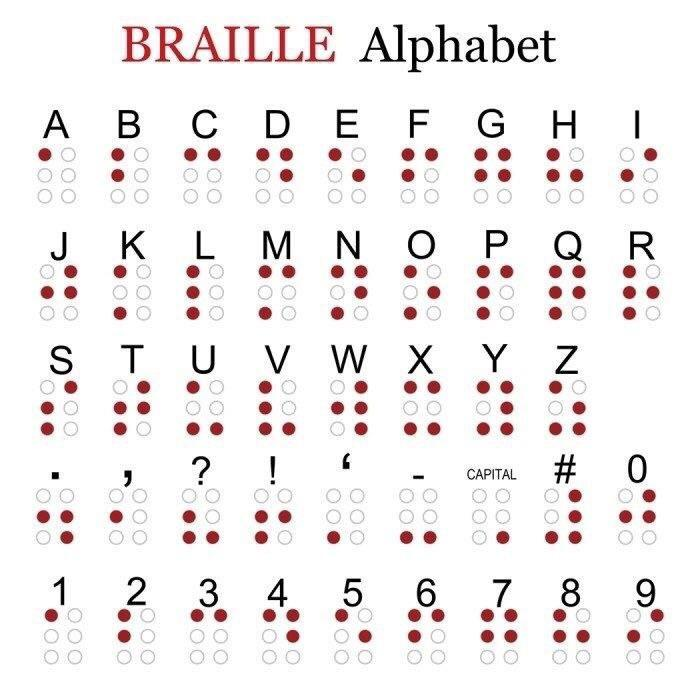
\includegraphics{read-braille.jpg}
%\end{figure}

    
\section*{Conclusion}
Morbi eleifend nibh euismod turpis convallis auctor. Phasellus sed interdum
turpis. Suspendisse condimentum sem non augue hendrerit consequat.
Pellentesque sodales nibh id leo scelerisque efficitur. Vestibulum maximus
leo non mollis ullamcorper\cite{Vogel:1979}. Fusce sit amet rutrum lacus. Integer id
malesuada diam, eget rutrum nisl. Nullam consequat neque id euismod
suscipit.

Nulla facilisi. Suspendisse varius, magna non blandit efficitur, dui purus
venenatis lorem, a sagittis lacus mauris molestie elit. Class aptent taciti
sociosqu ad litora torquent per conubia nostra, per inceptos himenaeos.
Nulla tellus nisi, auctor vehicula ipsum eu, tincidunt volutpat mauris.
Proin accumsan eget tellus vel semper. Nullam molestie pulvinar dolor sed
sollicitudin. Donec a porttitor ligula. Aenean sapien magna, interdum vitae
metus sed, sodales tristique magna. Integer sit amet dictum diam. Ut mi
nulla, ullamcorper porta vehicula dictum, blandit vel turpis.
    
\section*{Acknowledgements} UKM DCP-100-1000
    

\bibliographystyle{GayaUKM}
\bibliography{article}
\end{document}
